\documentclass{coupled}

\usepackage{graphicx}
\usepackage{amsmath}
\usepackage{amsfonts}
\usepackage{amssymb}

\usepackage[english]{babel}

\usepackage{listings}

\usepackage{pgf}
\usepackage{tikz}
\usepackage{pgfplots}

\usepackage{sidecap}
\usepackage{subfigure}

\usepackage{wrapfig}
\usepackage{amsmath}

\title{STABILITY OF COUPLING METHODS FOR CONJUGATE HEAT TRANSFER}

\author{SEBASTIAN T. SCHOLL$^{*}$, BART JANSSENS$^{\dag}$ AND TOM VERSTRAETE$^{\ddag}$}

\heading{Sebastian T. Scholl, Bart Janssens and Tom Verstraete}

\address{$^{*}$ $^{\ddag}$Von K\'{a}rm\'{a}n Institute for Fluid Dynamics\\
Chauss\'{e}e de Waterloo 72\\
1640 Rhode-St-Gen\`{e}se, Belgium\\
$^{*}$ e-mail: sebastian.scholl@vki.ac.be, web page: www.vki.ac.be\\
$^{\ddag}$ e-mail: tom.verstraete@vki.ac.be, web page: www.vki.ac.be
\and
$^{\dag}$Royal Military Academy\\
Renaissancelaan 30 \\
1000 Brussels, Belgium\\
e-mail: bart.janssens@rma.ac.be - web page: www.rma.ac.be}

\keywords{Conjugate Heat Transfer, Coupled Problems, Computing Methods, Stability}

\abstract{
We suggest a novel approach for coupled computations of conjugate heat transfer, considering the exchange of the boundary conditions between fluid and solid solver.
Within the multi-physics environment COOLFluiD 3, developed at the von K\'{a}rm\'{a}n Institute for Fluid Dynamics, we included four different coupling strategies. In all methods, boundary conditions are exchanged until equal temperatures and heat fluxes at the interface from the solid to the fluid domain. The first method sets a temperature distribution to the fluid solver that predicts a heat flux distribution imposed to the solid solver. %\cite{Verdicchio}. 
The second method sets a heat flux distribution to the fluid solver computing a temperature field for the solid. %\cite{Heidemann}. 
A third method imposes a temperature field to the fluid returning a Robin boundary condition to the solid using the wall heat transfer equation. % \cite{Montenay}. 
Based on a stability analysis for the existing coupling procedures, %\cite{Verstraete2008}, 
we postulate a new method, imposing a heat flux distribution to the fluid solver that returns a Robin boundary condition to the solid solver. % \cite{Verstraete2007}. 
The stability of all methods only depend on the dimensionless Biot number, the ratio of conductive to convective thermal resistance.
For flat plate computations, the result of each method is in good agreement with an analytical solution. We compare the novel coupling strategy with the established methods. Considering the stability, the new approach is advantageous, especially for high Biot numbers. Further, it converges faster concluding that it can improve efficiency and accuracy of conjugate heat transfer computations. 
}

\begin{document}
%\maketitle

\section{INTRODUCTION}
Many engineering design processes require to predict temperature distributions, e.g. the life of a turbine blade reduces by half with an increased metal temperature of 30 Kelvin \cite{Han}.  In case of a complex flow field, the temperature prediction is improved if the fluid and solid temperature computations are coupled. Besides the need for two different solvers, the challenge arises through the different time scales in the solid and the fluid that can vary by orders of magnitude and increase the computational cost. 

\section{NUMERICAL METHOD AND COUPLING PROCEDURES}

\subsection{EQUATIONS}

A displayed equation is numbered, using Arabic numbers in
parentheses. It should be centered, leaving a 6pt space above and
below to separate it from the surrounding text.

The following example is a single line equation:
\vskip-.6cm
\begin{eqnarray}
Ax = b
\end{eqnarray}

The next example is a multi-line equation:
\vskip-.6cm
\begin{eqnarray}
Ax = b \\
Ax = b \nonumber
\end{eqnarray}

\begin{table}[h!]
\caption{Example of the construction of one table}
\begin{center}
\begin{tabular}{*{3}{c}}
\hline
C11 & C12 & C13 \\
\hline
C21 & C22 & C23 \\
\hline
C31 & C32 & C33 \\
\hline
C41 & C42 & C43 \\
\hline
C51 & C52 & C53 \\
\hline
\end{tabular}
\end{center}
\end{table}
\section{STABILITY ANALYSIS}
\label{sec:STABILITY ANALYSIS}
All four methods have different stability and convergence properties.
We derived a stability criterion for coupled simulations of conjugate heat transfer, based on the relations between temperature and heat flux at the interface of solid and fluid domain \cite{Verstraete2008}.\\
Considering a one dimensional conjugate heat transfer problem, we specify a solid temperature at one boundary of the solid domain and the 
temperature of the fluid. The problem is to find the temperature $ T_{wall} $ and the heat flux $ q_{wall} $ at the interface. With the heat transfer coefficient $ h $, the thermal conductivity $ \lambda_{s} $ and the solid domain width $ L $ it is defined by:
\vskip-.6cm
\begin{eqnarray}
q_{wall} &=& \frac{\lambda_s}{L}(T_s - T_{wall}) \hspace{20mm} \text{on } \Omega_s, \\
q_{wall} &=& h(T_{wall} - T_{fluid})  \hspace{16mm} \text{on } \Omega_f, \nonumber
\end{eqnarray}
representing heat fluxes resulting from the solid domain ($ \Omega_s $) and the fluid domain ($ \Omega_f $) computations. Heat fluxes equal at the interface and we have:
\vskip-.6cm
\begin{eqnarray}
\frac{\lambda_s}{L}(T_s-T_{wall}) &=& h(T_{wall}-T_{fluid}).
\end{eqnarray}
With the Biot number $ Bi=\frac{hL}{\lambda_s} $ the previous equation becomes:
\vskip-.6cm
\begin{eqnarray}
T_s-T_{wall}&=&Bi(T_{wall}-T_{fluid}).
\end{eqnarray}
Thus, the wall temperature is:\\
\vskip-.6cm
\begin{eqnarray}
T_{wall} &=& \frac{Ts+Bi \cdot T_{fluid}}{1+Bi}.
\end{eqnarray}
In the next sections, we continue with the stability analysis for each of the four methods.

\subsection{STABILITY OF THE FFTB METHOD}

In the FFTB method, a wall temperature $ T_{wall}^{0} $ is imposed to the fluid domain that varys by a value $ \alpha_0 $ from the correct wall temperature:
\vskip-.6cm
\begin{eqnarray}
T_{wall}^0 &=& T_{wall} + \alpha_{0}.
\end{eqnarray}
The heat flux solid is then:
\vskip-.6cm
\begin{eqnarray}
q_{wall}^0 &=& h(T_{wall}^0 - T_{fluid})\\
&=& h(T_{wall}-T_{fluid})+h\cdot \alpha_{0}\nonumber \\
&=& q_{wall} +h\alpha_{0} .\nonumber
\end{eqnarray}
Using the new heat flux imposed to the solid results in a new wall temperature:
\vskip-.6cm
\begin{eqnarray}
T_{wall}^{1}&=&T_s-\frac{L}{\lambda_{s}} \cdot q_{wall}^0\\
&=& T_s - \frac{L}{\lambda_{s}} \cdot q_{wall} - \alpha^{0} \frac{hL}{\lambda_{s}}\nonumber \\
&=& T_{wall} - \alpha_{0} \cdot Bi.
\end{eqnarray}
At the i-th iteration, the temperature is given by:
\vskip-.6cm
\begin{eqnarray}
T_{wall}^{i}&=&T_{wall}+\alpha_{0} \cdot (-Bi)^{i}.
\end{eqnarray}
The heat flux results in:
\vskip-.6cm
\begin{eqnarray}
q_{wall}^{i}&=&q_{wall}+\alpha_{0} \cdot (-Bi)^{i} \cdot h.
\end{eqnarray}
As we can see, convergence is only achieved, if $ |Bi| < 1 $.

\subsection{STABILITY OF THE TFFB METHOD}

In the TFFB method, a wall temperature $ T_{wall}^{0} $ is imposed to the solid domain that varys by a value $ \alpha_0 $ from the correct wall temperature:
\vskip-.6cm
\begin{eqnarray}
T_{wall}^0 &=& T_{wall} + \alpha_{0}.
\end{eqnarray}
The heat flux is then:
\vskip-.6cm
\begin{eqnarray}
q_{wall}^0 &=& \frac{\lambda_{s}}{L}(T_{s} - T_{wall}^0)\\
&=& \frac{\lambda_{s}}{L}(T_{s} - T_{wall})+\frac{\lambda_{s}}{L} \cdot \alpha_{0}\nonumber \\
&=& q_{wall} +\frac{\lambda_{s}}{L}\alpha_{0} .\nonumber
\end{eqnarray}
Using the new heat flux imposed to the fluid results in a new wall temperature:
\vskip-.6cm
\begin{eqnarray}
T_{wall}^{1}&=&T_{fluid}+\frac{q_{wall}^{0}}{h}\\
&=& T_{fluid}+\frac{q_{wall}}{h} - \alpha^{0} \frac{\lambda_{s}}{hL}\nonumber \\
&=& T_{wall} - \frac{\alpha_{0}}{Bi}.
\end{eqnarray}
At the i-th iteration, the temperature is given by:
\vskip-.6cm
\begin{eqnarray}
T_{wall}^{i}&=&T_{wall}+\alpha_{0} \cdot \left(-\frac{1}{Bi}\right)^{i}.
\end{eqnarray}
The heat flux results in:
\vskip-.6cm
\begin{eqnarray}
q_{wall}^{i}&=&q_{wall}+\alpha_{0} \cdot \left(-\frac{1}{Bi}\right)^{i} \cdot \frac{\lambda_{s}}{L}.
\end{eqnarray}
As we can see, convergence is only achieved, if $ |Bi| > 1 $.

\subsection{STABILITY OF THE hFTB METHOD}

\subsection{STABILITY OF THE hFFB METHOD}

\section{FLAT PLATE TEST CASE}

Schematic diagram for conjugate heat transfer test case:\\

\begin{figure}[th!]
\subfigure[Grid dependence study with normalized temperature.]{
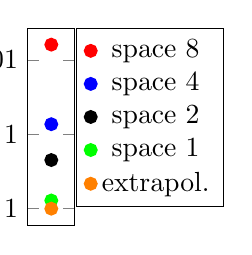
\begin{tikzpicture}[baseline,trim axis left]
\begin{axis}[ at={(0pt,0pt)}, name=plot, xlabel=  ,ylabel= T, legend pos=outer north east, width=0.6cm,scale only axis,height=2.5cm,
xtick=\empty]
\addplot[color=red, mark=*, only marks, line width=1pt] plot coordinates {
    (1,4.0879768830/4.043359014)
};
\addplot[color=blue, mark=*, only marks, line width=1pt] plot coordinates {
    (1,4.0662876068/4.043359014)
};
\addplot[color=black, mark=*, only marks, line width=1pt] plot coordinates {
    (1,4.0565397534/4.043359014)
};
\addplot[color=green, mark=*, only marks, line width=1pt] plot coordinates {
    (1,4.0455946121/4.043359014)
};
\addplot[color=orange, mark=*, only marks, line width=1pt] plot coordinates {
    (1,4.043359014/4.043359014)
};
\legend{space 8,space 4,space 2,space 1, extrapol.}
\end{axis}
\end{tikzpicture}
    \label{fig:subfig1}
}
\subfigure[Grid, space 8.]{
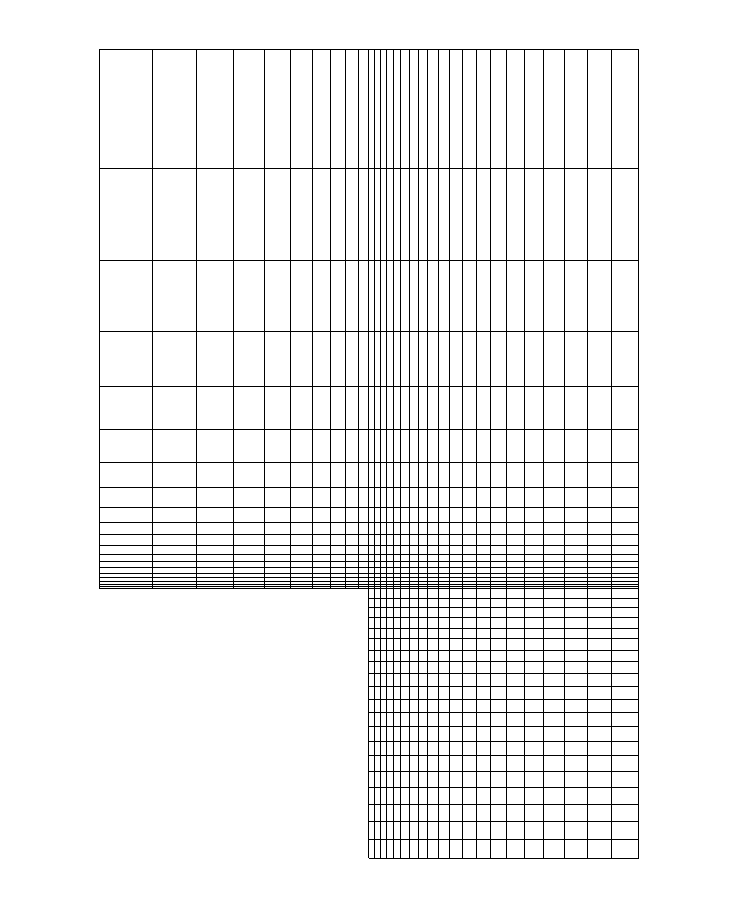
\includegraphics[trim=0cm 0cm 0cm 0cm, width=4cm]{figures/grid4.png}
    \label{fig:subfig2}
}
\subfigure[Flat plate.]{
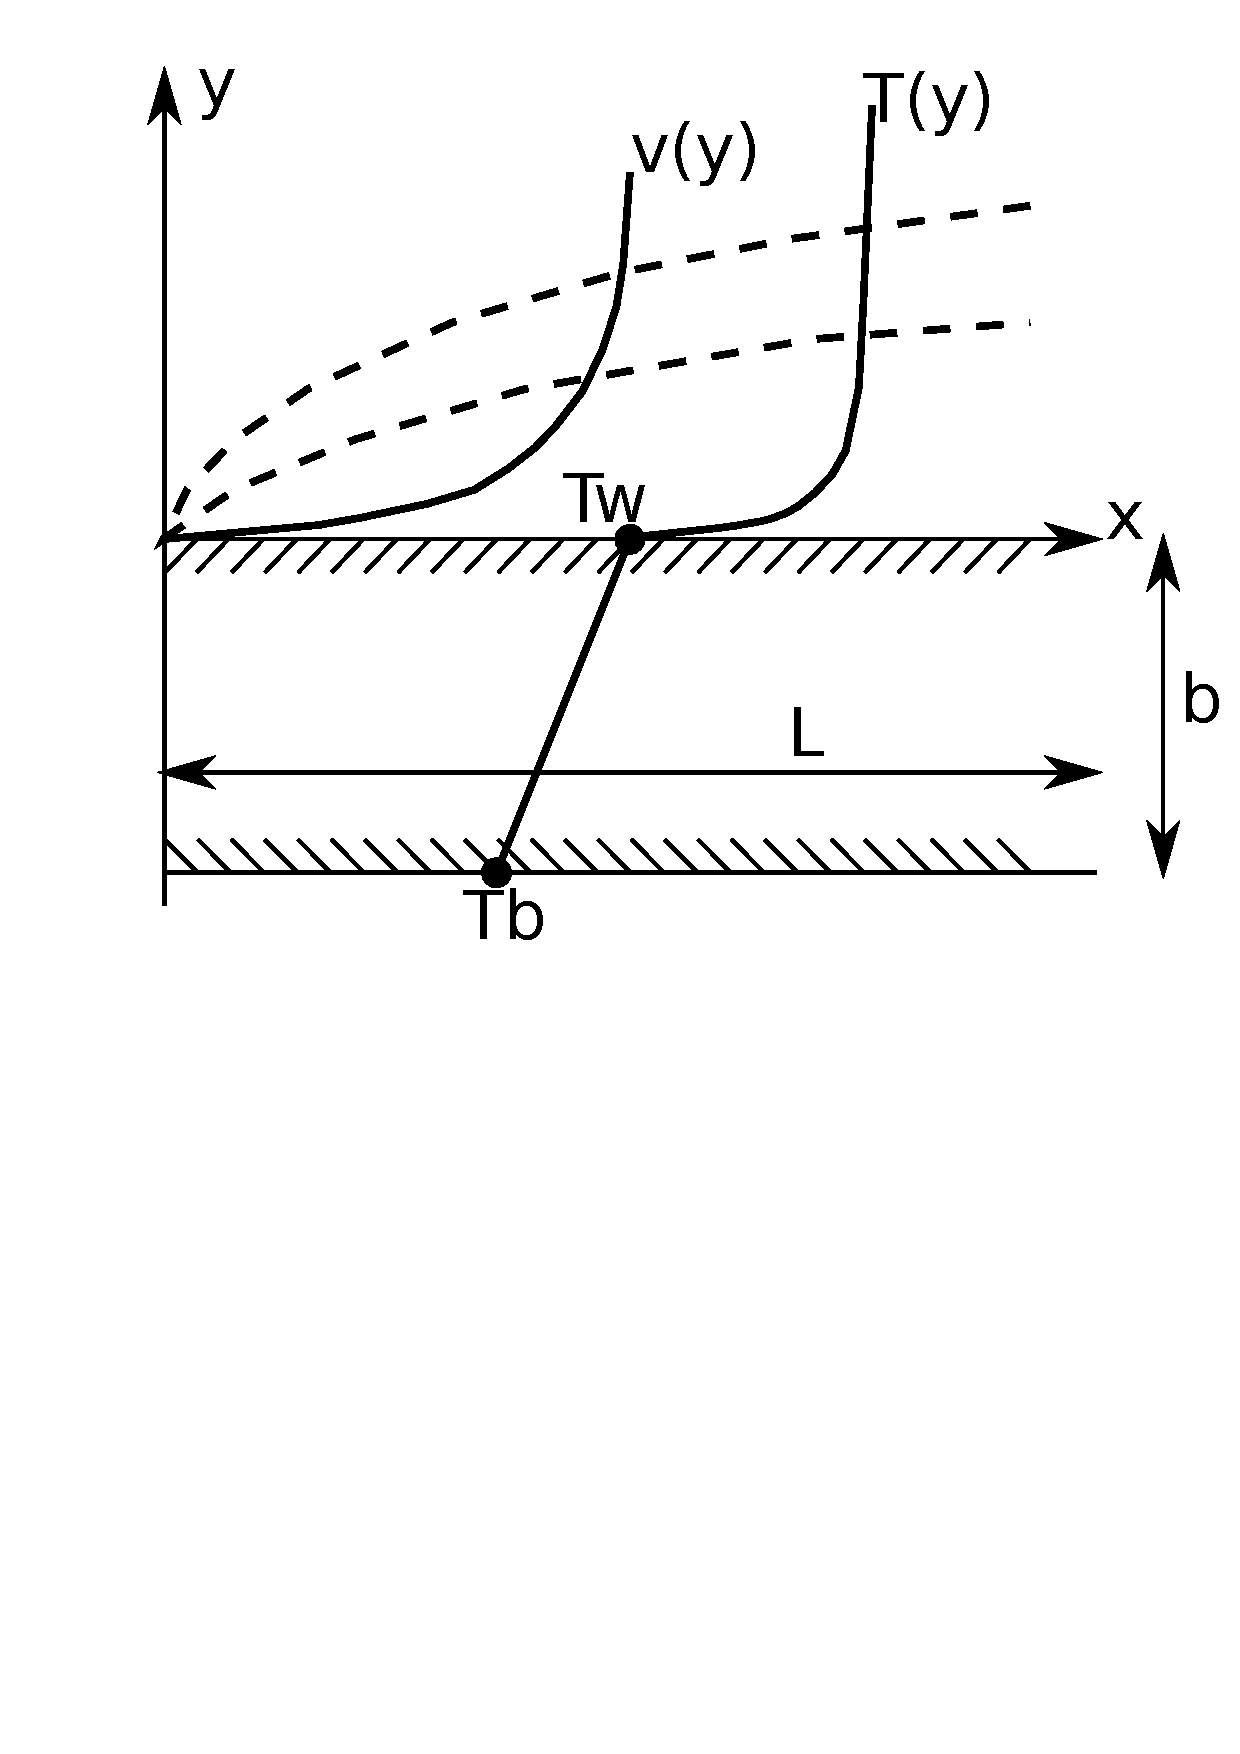
\includegraphics[trim = 10mm 120mm 20mm 5mm, width=4cm]{figures/Luikov4.pdf}
    \label{fig:subfig3}
}
  \caption{Grid for computational setup.}
\end{figure}
\newpage

\section{RESULTS AND DISCUSSION}
\begin{figure}[th!]
\subfigure[One fluid solve per iteration.]{
    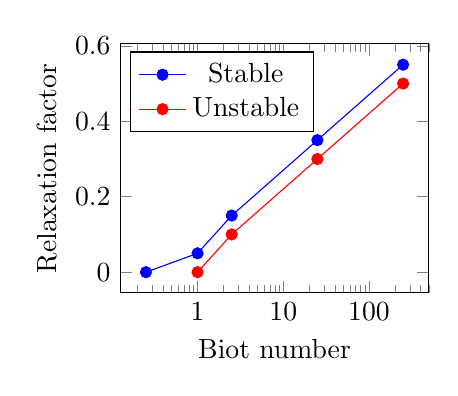
\begin{tikzpicture}
\begin{semilogxaxis}[width=55mm,
	%title={FFTB stability},
	legend pos=north west,
    unbounded coords=discard,
    log basis x=10,
    log ticks with fixed point
    ,xlabel=Biot number,ylabel=Relaxation factor]
\addplot[blue, mark=*] coordinates {
(0.25,
0.00)
(1,
0.05)
(2.5,
0.15)
(25,
0.35)
(250,
0.55)
};
\addplot[red, mark=*]  coordinates {
(1,
0.00)
(2.5,
0.10)
(25,
0.30)
(250,
0.50)
};
\legend{Stable,Unstable}
\end{semilogxaxis}
\end{tikzpicture}
    \label{fig:subfig1}
}
\subfigure[Ten fluid solves per iteration.]{
    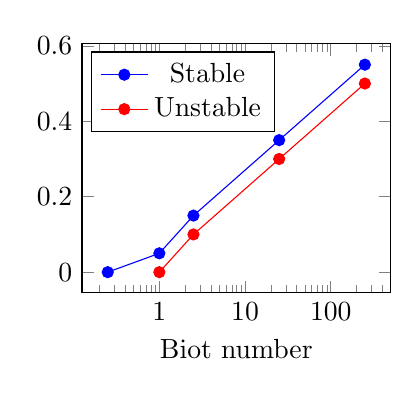
\begin{tikzpicture}
\begin{semilogxaxis}[width=55mm,
	%title={FFTB stability},
	legend pos=north west,
    unbounded coords=discard,
    log basis x=10,
    log ticks with fixed point
    ,xlabel=Biot number,ylabel=]
\addplot[blue, mark=*] coordinates {
(0.25,
0.00)
(1,
0.05)
(2.5,
0.15)
(25,
0.35)
(250,
0.55)
};
\addplot[red, mark=*]  coordinates {
(1,
0.00)
(2.5,
0.10)
(25,
0.30)
(250,
0.50)
};
\legend{Stable,Unstable}
\end{semilogxaxis}
\end{tikzpicture}
    \label{fig:subfig2}
}
\subfigure[100 fluid solves per iteration.]{
    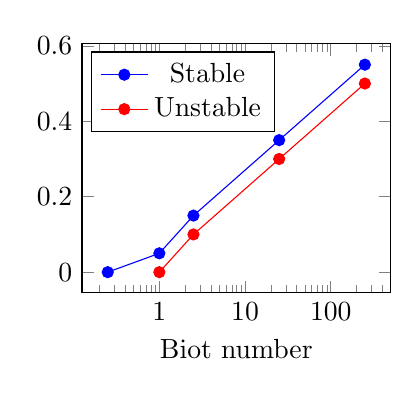
\begin{tikzpicture}
\begin{semilogxaxis}[width=55mm,
	%title={FFTB stability},
	legend pos=north west,
    unbounded coords=discard,
    log basis x=10,
    log ticks with fixed point
    ,xlabel=Biot number,ylabel=]
\addplot[blue, mark=*] coordinates {
(0.25,
0.00)
(1,
0.05)
(2.5,
0.15)
(25,
0.35)
(250,
0.55)
};
\addplot[red, mark=*]  coordinates {
(1,
0.00)
(2.5,
0.10)
(25,
0.30)
(250,
0.50)
};
\legend{Stable,Unstable}
\end{semilogxaxis}
\end{tikzpicture}
    \label{fig:subfig3}
}
  \caption{Stability of the FFTB method as a function of the Biot number for different fluid solves per iteration.}
\end{figure}

\section{CONCLUSIONS}
\begin{itemize}
\item found a stability criterion for cht computations
\item confirm the stability criterion, dependence on Biot number by validation flat plate test case
\item influence of Navier-Stokes computations per iteration
\item one coupling procedure (hFTB) does not converge as the others
\item flux back methods converge faster for many Navier-Stokes solves per iteration
\item suggest a novel coupling procedure
\end{itemize}


\section*{ACKNOWLEDGEMENTS}

The research leading to this results has received funding from the European's Comunnity's Seventh Framework Programme (FP7, 2007-2013), PEOPLE programme, under the grant agreement No. FP7-290042 (COPA-GT project).

\begin{thebibliography}{99}

\bibitem{Han} J.-C. Han, S. Dutta and S. Ekkad, \textit{Gas turbine heat transfer and cooling technology}. Taylor and Francis, 2001.
%\bibitem{Verdicchio} J.A. Verdicchio, J.W. Chew and N.J. Hills, “Coupled Fluid/Solid Heat Transfer Computation for Turbine Discs”, ASME %Paper No. 2001-GT-0205.
%\bibitem{Heidemann} J.D. Heidemann, A.J. Kassab, E.A. Divo, F. Rodriguez and E. Steinthorsson, “Conjugate Heat Transfer Effects on a %Realistic Film-Cooled Turbine Vane”. ASME TURBO EXPO, No.GT2033-38553.
%\bibitem{Montenay} A. Montenay, L. Paté and J. Duboué, “Conjugate Heat Transfer Analysis of an Engine Internal Cavity” ASME Paper No. %2000-GT-282.
\bibitem{Verstraete2008} T. Verstraete, “Multidisciplinary Turbomachinery Component Optimization Considering Performance, Stress, and Internal Heat Transfer”, PhD-Thesis, Universiteit Gent, 2008.
\bibitem{Verstraete2007} T. Verstraete, Z. Alsalihi and R. A. Van den Braembussche, “Numerical Study of the Heat Transfer in Micro Gas Turbines”, J. of Turbomachinery, Vol. 129, pp. 835-841, 2007.

%\bibitem{Zienkiewicz}  Zienkiewicz, O.C. and  Taylor, R.L. \textit{The finite element method}. McGraw Hill,
%Vol. I., (1989), Vol. II., (1991).
%\bibitem{Idelsohn} Idelsohn, S.R. and O\~{n}ate, E. Finite element and finite volumes. Two good friends.
%\textit{Int. J. Num. Meth. Engng.} (1994) \textbf{37}:3323--3341.

\end{thebibliography}

\end{document}


